\documentclass[10pt,twocolumn,letterpaper]{article}

\usepackage{acvs}
\usepackage{times}
\usepackage{epsfig}
\usepackage{graphicx}
\usepackage{amsmath}
\usepackage{amssymb}

% Include other packages here, before hyperref.
\usepackage{dsfont}

% If you comment hyperref and then uncomment it, you should delete
% egpaper.aux before re-running latex.  (Or just hit 'q' on the first latex
% run, let it finish, and you should be clear).
\usepackage[pagebackref=true,breaklinks=true,letterpaper=true,colorlinks,bookmarks=false]{hyperref}

\iccvfinalcopy % *** Uncomment this line for the final submission

\def\iccvPaperID{} % *** Enter the Paper ID here
\def\httilde{\mbox{\tt\raisebox{-.5ex}{\symbol{126}}}}

% Pages are numbered in submission mode, and unnumbered in camera-ready
\ificcvfinal\pagestyle{empty}\fi

\begin{document}

%%%%%%%%% TITLE - PLEASE UPDATE
\title{Deformable DETR: Deformable Transformers for End-to-End Object Detection~\cite{deformabledetr} \\ {\rm {\normalsize Minji Kim (minji@snu.ac.kr; 2020-28702), Dept. of Electrical and Computer Engineering, Seoul National University}}}   % **** Enter the paper title and student information here

\maketitle
\thispagestyle{empty}

%%%%%%%%% BODY TEXT - ENTER YOUR RESPONSE BELOW

%%%%%%%%%%%%%%%%%
%%%%%%%%%%%%%%%%%
\section{Introduction}
Despite the straightforward design of DETR~\cite{detr} which enables to remove many hand-crafted components such as anchor generation, pseudo target assignment, and non-maximum suppression (NMS), there are two inherent drawbacks in DETR: 1) slow convergence and 2) low performance on small objects.
DETR computes self-attention in all possible regions, which results in higher computational cost and slower convergence during training compared to traditional CNN-based object detection models.
Furthermore, this kind of heavy computation in DETR makes it difficult to use high-resolution feature maps, whereas recent CNN detection models mostly adopt multi-scale features to detect small objects.
As an alternative, Deformable DETR adopts a deformable attention module which significantly reduces computation and learning time by considering only the main sampling points near the learned reference coordinates.
In addition, the detection performance of small objects is enhanced by utilizing high-resolution feature maps by cross-attention between multi-scale feature maps.



%%%%%%%%%%%%%%%%%
%%%%%%%%%%%%%%%%%
\section{Deformable DETR}

Fig.~\ref{fig:overview} shows the overall architecture of Deformable DETR.

\subsection{Deformable Attention Module}
Inspired by deformable convolution~\cite{deformablecnn}, the deformable attention module only attends to a small set of key sampling points nearby a reference point.
Given a feature map $x \in \mathbb{R}^{C \times H \times W}$, a content feature $z_q$, and a reference point $p_q$ where $q$ indexing a query element, the deformable attention is calculated as follows:
\begin{equation}
\begin{split}
    & \textrm{DeformAttn}(z_q, p_q, x) \\
    & = \sum^{M}_{m=1}W_m[\sum^{K}_{k=1}A_{mqk} \cdot W_m'x(p_q + \Delta  p_mqk)],
\end{split}
\end{equation}
where $m$ and $k$ indexes the attention head and sampled keys, respectively.
Note that the total sampled key number $K$ is much smaller than DETR where each pixel location in feature map becomes a sampling point ($K << HW$).
This operation is applied for multi-scale layers of feature maps from the backbone, \eg, $C_3$ through $C_5$ in ResNet.
The top-down structure in standard Feature Pyramid Networks is not adopted.

\subsection{Two-Stage Deformable DETR}
This version uses the generated region proposals from the first stage as object queries for further refinement.
Specifically, the encoder part of Deformable DETR first produces a region proposals with regarding each location in multi-scale feature maps as an object query, and then the top scoring bounding boxes are picked as region proposals.




%%%%%%%%%%%%%%%%%
%%%%%%%%%%%%%%%%%
\section{Personal Notes}

Deformable DETR reduces the training GPU hours of DETR from 2000 hours to ~300 hours on COCO 2017 dataset.
In practice, this is still slow when compared to the detector with CNN architectures.
Furthermore, the performance of Deformable DETR is still far lower then other state-of-the-art models.
I've searched follow-up studies which mainly focuses on reducing the training costs and achieving the performance boosts; none of them was interesting as these kinds of efforts tend to harm the soul of DETR which aims to remove the hand-crafted components.


\begin{figure}[t]
    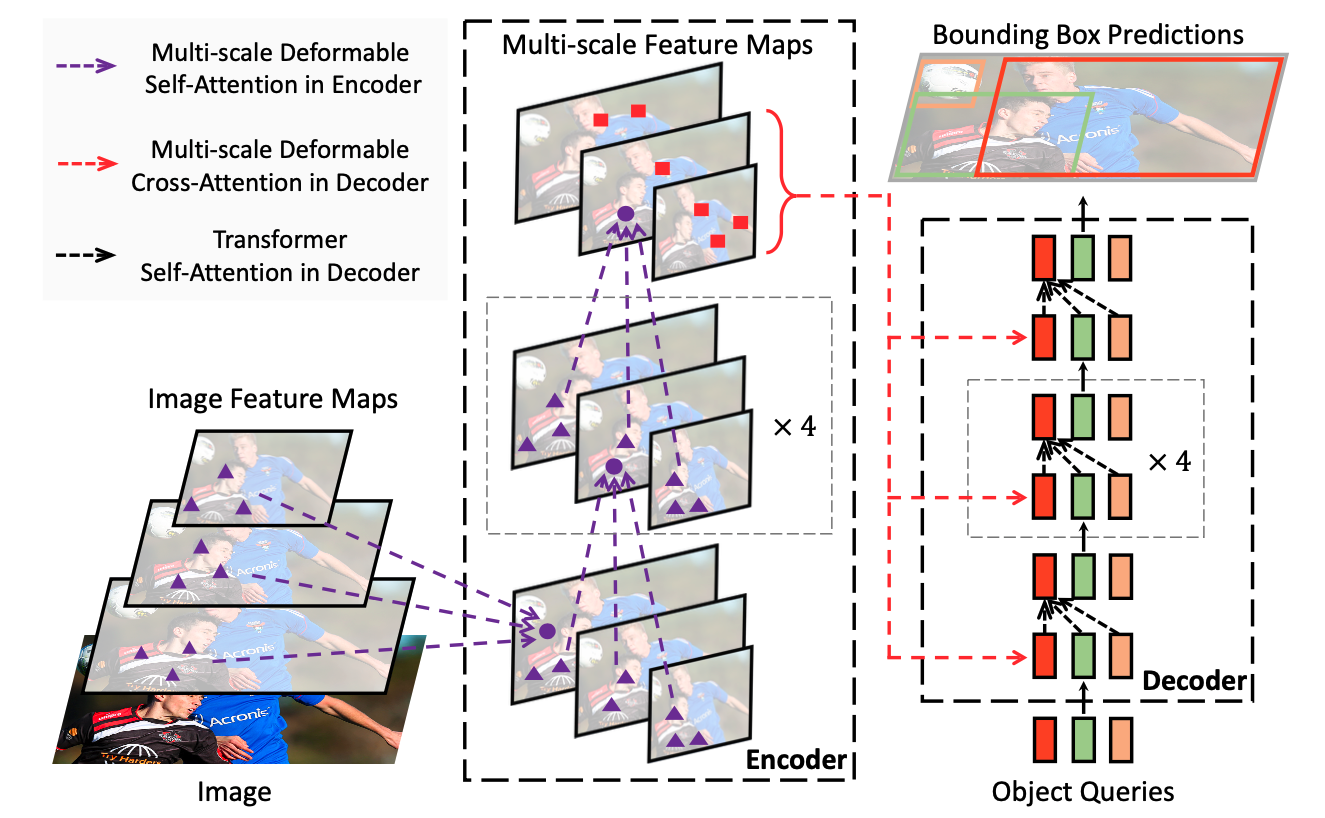
\includegraphics[width=\linewidth]{assets/deformable_detr.png}
    \caption{\label{fig:overview}The overall pipeline of Deformable DETR.}
\end{figure}



{\small
\bibliographystyle{ieee}
\bibliography{egbib}
}

\end{document}
